\section{System Design}

\subsection{Functional Requirements}
The Student Life Support Service is designed to fulfill the specific functional requirements of three key user roles: Students, Dormitory Staff (or Student Affairs), and Administrators. Each role has its own set of features tailored to its needs within the system.

\noindent \textbf{User Type}: S-Student, DS-Dormitory Staff/Student Affairs, A-Admin (Operator) \\
\textbf{Categorized}: F-Functional, NF-Nonfunctional

\newcolumntype{L}{>{\arraybackslash}m{3.5cm}}
\begin{longtable}{|m{0.6cm}|m{2.8cm}|m{5.4cm}|m{1.6cm}|m{1.5cm}|m{1.8cm}|}
	\hline
	\textbf{No} & \textbf{Requirement }             & \textbf{Description}                                                                                          & \textbf{Priority} & \textbf{User Type}  & \textbf{Category} \\ \hline
	\endhead
	1  & Manage personal info     & Users can view and update their personal information.                                                 & Medium   & S, DS, A   & F           \\ \hline
	2  & Support tickets          & Users can create (raise), view support tickets.                                                       & High     & S, DS, A   & F           \\ \hline
	3  & Contact through messages & Users can contact the staff or students handling the support ticket through text messages.            & High     & S, DS      & F           \\ \hline
	4  & Ticket rating            & Students can rate their tickets which are marked as done.                                             & Medium   & S          & F           \\ \hline
	5  & View newsfeed            & Users can view a newsfeed of public pending/in-process tickets.                                        & Low      & S, DS, A   & F           \\ \hline
	6  & View notifications       & Users can view notifications and announcements.                                                       & Medium   & S, DS, A   & F           \\ \hline
	7  & Feedback and suggestions & Users can give feedback and suggestions for the system.                                                & Medium   & S, DS, A   & F          \\ \hline
	8  & Handle support tickets   & Dormitory staff can view and handle (mark as done, cancel) support tickets.                            & High     & DS         & F           \\ \hline
	9  & View past tickets        & Dormitory staff can view all previously handled support tickets.                                       & Medium   & DS         & F           \\ \hline
	10 & Manage notifications     & Dormitory staff and admins can create and manage notifications and announcements.                      & High     & DS, A      & F           \\ \hline
	11 & Manage users             & Admins can manage all users/roles (create, view, update, delete).                                      & High     & A          & F           \\ \hline
	12 & Manage tickets           & Admins can manage all support tickets (view, delete).                                                  & High     & A          & F           \\ \hline
	13 & Manage dormitories       & Admins can manage all dormitories (create, view, delete).                                              & Medium   & A          & F           \\ \hline
	14 & Manage system logs       & Admins can manage system logs (view, delete).                                                          & Medium   & A          & F           \\ \hline
	15 & Manage feedback          & Admins can manage system feedback (view, delete).                                                      & Low      & A          & F           \\ \hline
	16 & View system report       & Admins can generate and view system reports.                                                           & High     & A          & F           \\ \hline
	
	
	\caption{Functional Requirements}
	\label{tab:functionalRequirement}
\end{longtable}


For clearer comprehension, the table presented below provides a detailed visualization of the functional requirements, organized according to the different user roles within the system. This structure allows for a more precise understanding of how each role interacts with the system's features and capabilities.

\begin{longtable}{{|m{4.8cm}|m{12cm}|}} 
	\hline
	\textbf{User roles} & \textbf{Functional Requirements}\\ \hline
	\endhead
	
	Student & 	
	\begin{itemize}
		\item can view, update his/her personal information.
		\item can create (raise), view his/her support tickets. 
		\item can contact the staff who handles the support ticket through text messages.
		\item can rate his/her tickets which are marked as done.
		\item can view newsfeed (public pending/in process tickets).
		\item can view notifications, announcement.
		\item can give feedback and suggestions for the system.
	\end{itemize}
	
	\\ \hline
	
	Dormitory staff/ Student Affairs & 	
	\begin{itemize}
		\item can view, update his/her personal information.
		\item can view all available support tickets.
		\item can handle support tickets. (mark as done, cancelled)
		\item can view all past handled tickets.
		\item can contact students who owns the ticket through text messages.
		\item can view newsfeed (public pending/in process tickets).
		\item can create, view notifications, announcement. 
		\item can give feedback and suggestions for the system.
	\end{itemize}
	
	\\ \hline
	
	
	Admin (Operator) & 	
	\begin{itemize}
		\item can manage his/her personal information (view, update).
		\item can manage all users/roles (create, view, update, delete).
		\item can manage all support tickets (view, delete).
		\item can manage all dormitories (create, view, delete).
		\item can manage system logs (view, delete).
		\item can manage system feedback (view, delete).
		\item can view newsfeed (public pending/in process tickets).
		\item can manage notifications, announcement (create, view). 
		\item can view the system report.
	\end{itemize}
	
	\\ \hline
	
	
	\caption{Functional Requirements by User Roles} % needs to go inside longtable environment
	\label{tab:functionalRequirements}
\end{longtable}



\subsection{Non-Functional Requirements}
\noindent \textbf{Categorized}: NF-Nonfunctional

\newcolumntype{L}{>{\arraybackslash}m{3.5cm}}



	\begin{longtable}{|m{0.5cm}|m{2.5cm}|m{7cm}|m{1.5cm}|m{1.7cm}|m{2.4cm}|}
		\hline
		\textbf{No} & \textbf{Requirement}                & \textbf{Description}                                                                                                                               & \textbf{Priority} & \textbf{Category}  & \textbf{Functioning} \\ \hline
		\endhead
		1  & Fast Response Time          & The system should provide fast responses for user interactions such as submitting tickets, viewing statuses, and real-time messaging.      & High     & NF        & Performance \\ \hline
		2  & Real-Time Communication     & Messages between students and staff should be transmitted with minimal latency (under 100 milliseconds).                                   & High     & NF        & Performance \\ \hline
		3  & Concurrent Users            & The system must support up to 500 concurrent users without significant performance degradation.                                            & High     & NF        & Performance \\ \hline
		4  & Database Query Optimization & PostgreSQL database should be optimized to handle high read/write volume efficiently even during peak load.                                & High     & NF        & Performance \\ \hline
		5  & JWT-Based Authentication    & Secure authentication using JSON Web Tokens (JWT), with short-lived tokens and securely stored refresh tokens in Redis.                    & High     & NF        & Security    \\ \hline
		6  & Role-Based Access Control   & Enforce strict role-based access to ensure users only have access to the functionality appropriate for their role.                         & High     & NF        & Security    \\ \hline
		7  & Encryption                  & All communications between the client and server must be encrypted using HTTPS to ensure data security.                                    & High     & NF        & Security    \\ \hline
		8  & Data Validation             & Input from users must be validated and sanitized to protect against common vulnerabilities like SQL Injection and Cross-Site Scripting.     & High     & NF        & Security    \\ \hline
		9  & Audit Logs                  & Admins must have access to immutable and secure audit logs to track user actions such as login attempts and system modifications.           & Medium   & NF        & Security    \\ \hline
		10 & Database Scalability        & The PostgreSQL database should scale efficiently as the number of tickets, messages, and users grows.                                       & High     & NF        & Scalability \\ \hline
		11 & User-Friendly Interface     & The interface should be intuitive and easy to navigate for users of varying technical abilities.                                            & High     & NF        & Usability   \\ \hline
		12 & Cross-Device Compatibility  & The system should be responsive and function well on desktops, laptops, tablets, and smartphones.                                           & High     & NF        & Usability   \\ \hline
	
		\caption{Non-Functional Requirements}
	\label{tab:nonfunctionalRequirements}
	
	\end{longtable}



\subsection{Use Case Diagrams}
	\begin{figure}[H]
		\centering
		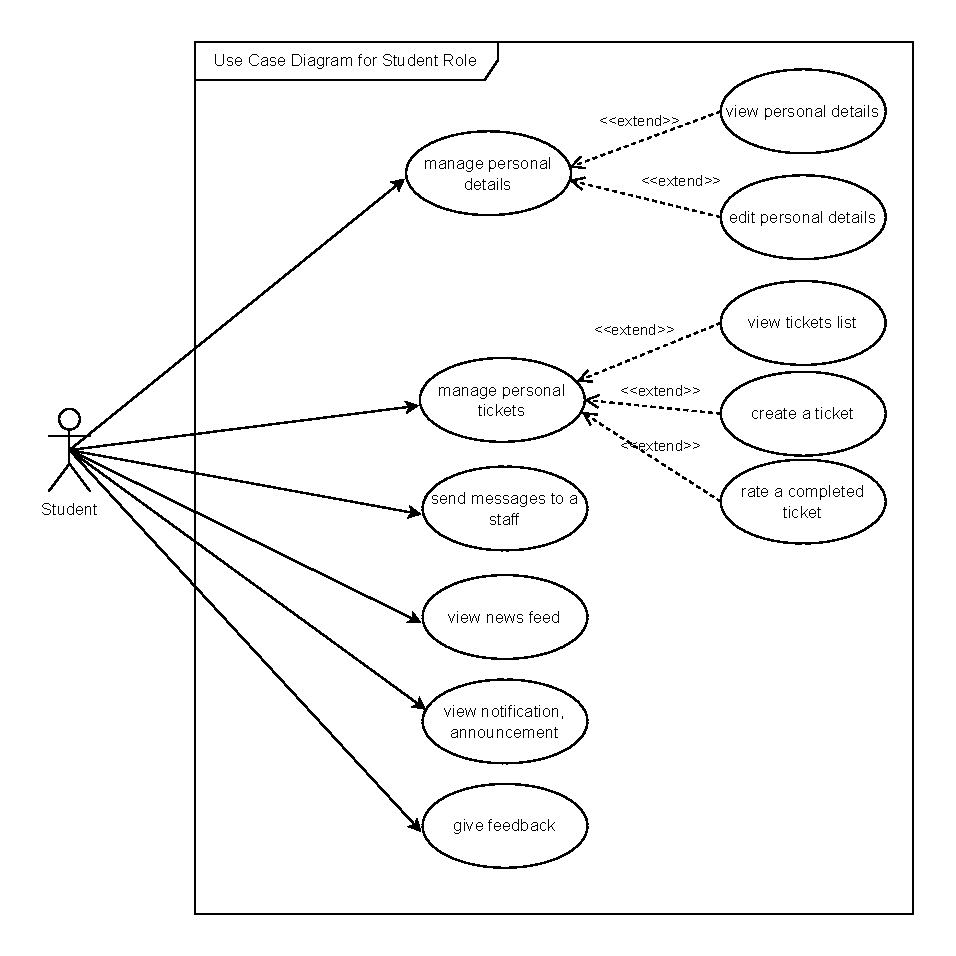
\includegraphics[width=0.82\columnwidth]{graphics/student use case.pdf}
		\caption{Student Use Case Diagram}
		\label{fig:student-use-case}
	\end{figure}
	
	
	
	\begin{figure}[H]
		\centering
		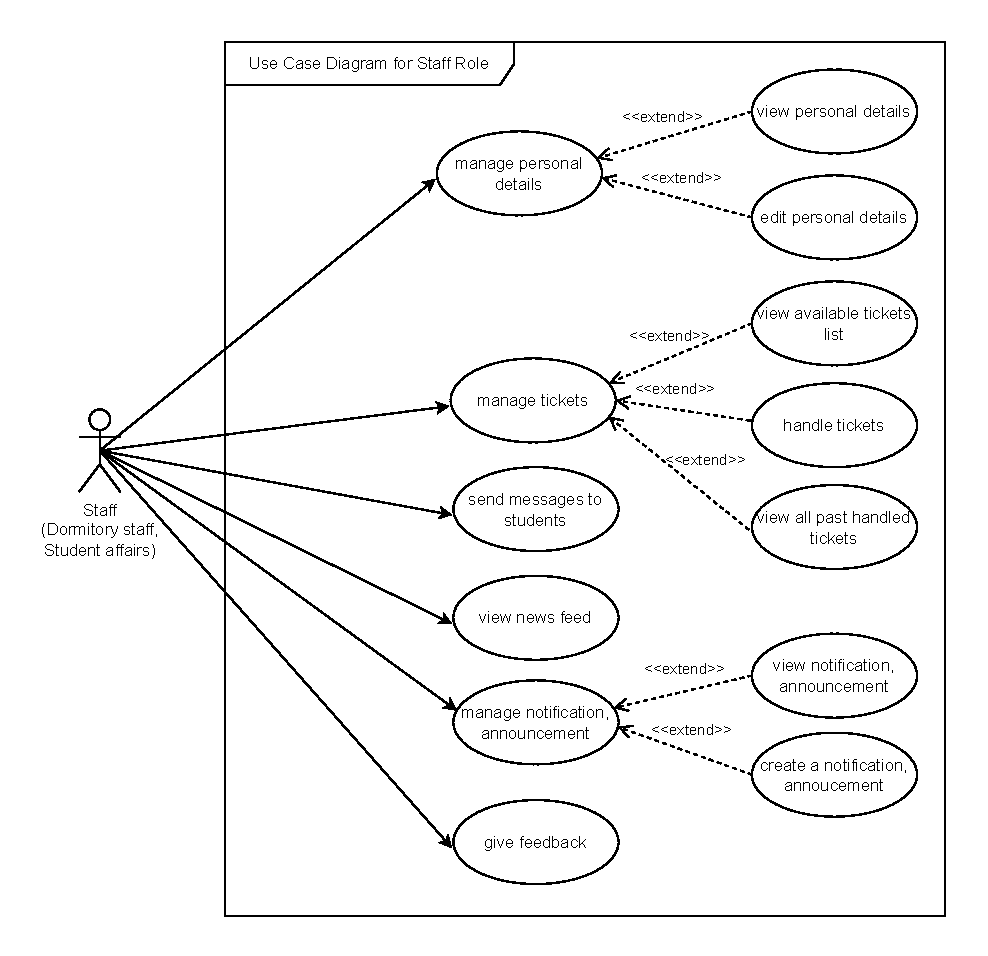
\includegraphics[width=0.9\columnwidth]{graphics/staff use case.pdf}
		\caption{Staff (Dormitory staff, Student affairs) Use Case Diagram}
		\label{fig:staff-use-case}
	\end{figure}
	
	
	
	\begin{figure}[H]
		\centering
		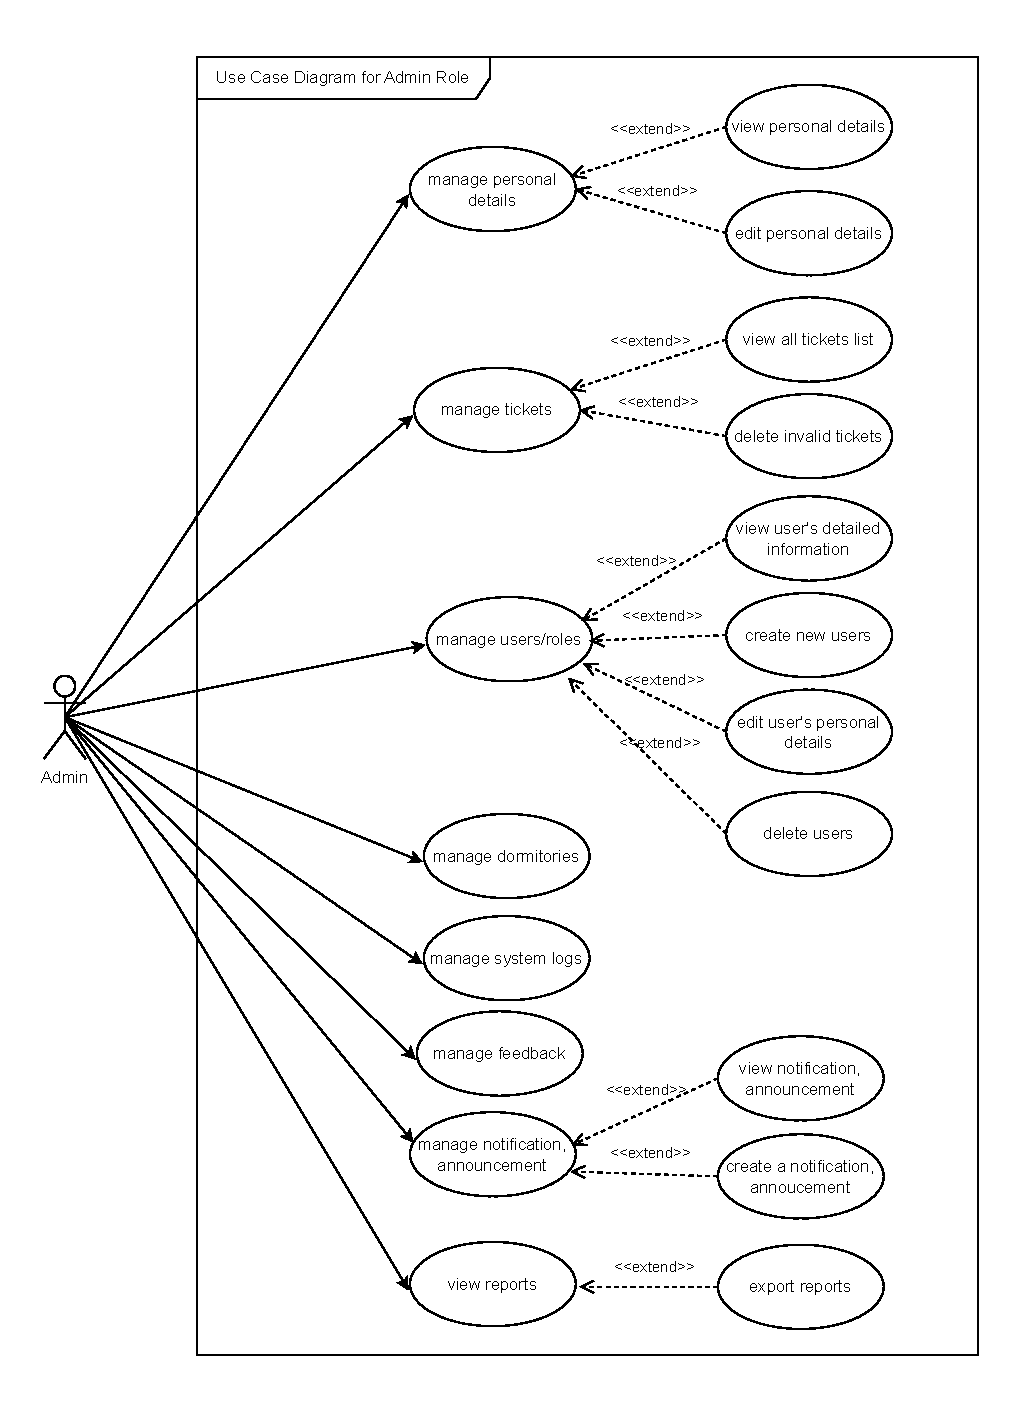
\includegraphics[width=0.84\columnwidth]{graphics/admin-use-case.pdf}
		\caption{Admin Use Case Diagram}
		\label{fig:admin-use-case}
	\end{figure}
	
	
\subsection{Process Workflow Diagrams}	
The core functionality of the Student Life Support Service is its ticket-raising process. The following diagram provides a detailed step-by-step illustration of this process.


\begin{figure}[H]
	\centering
	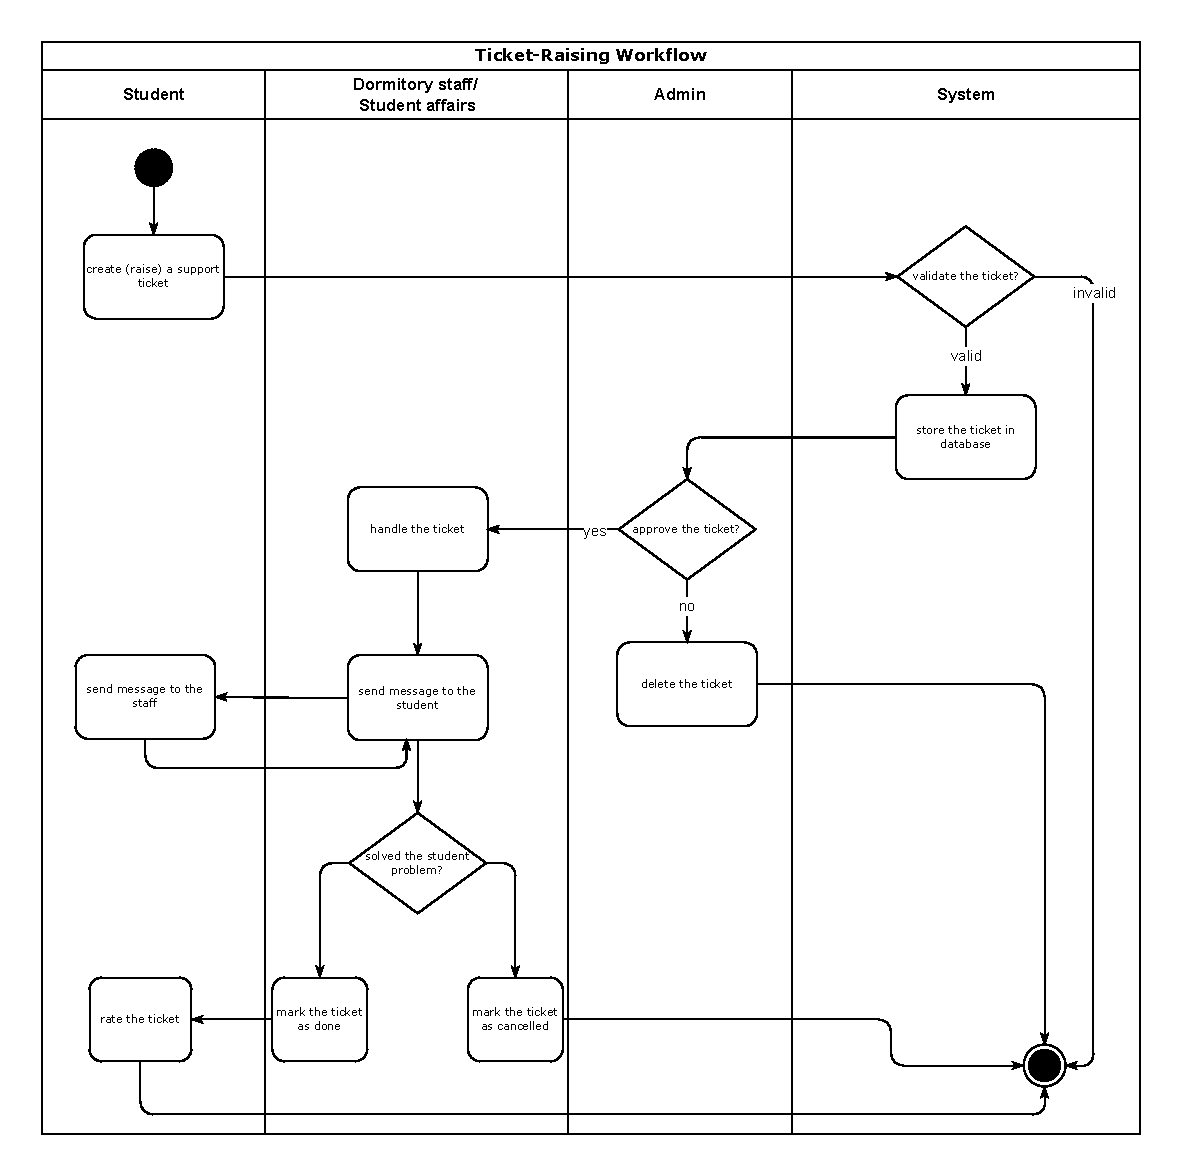
\includegraphics[width=0.84\columnwidth]{graphics/sys-workflow.pdf}
	\caption{Ticket-Raising Process Workflow}
	\label{fig:ticket-raising-workflow}
\end{figure}


\subsection{Database Design}
	\subsubsection{ER Diagram}
	\begin{figure}[H]
		\centering
		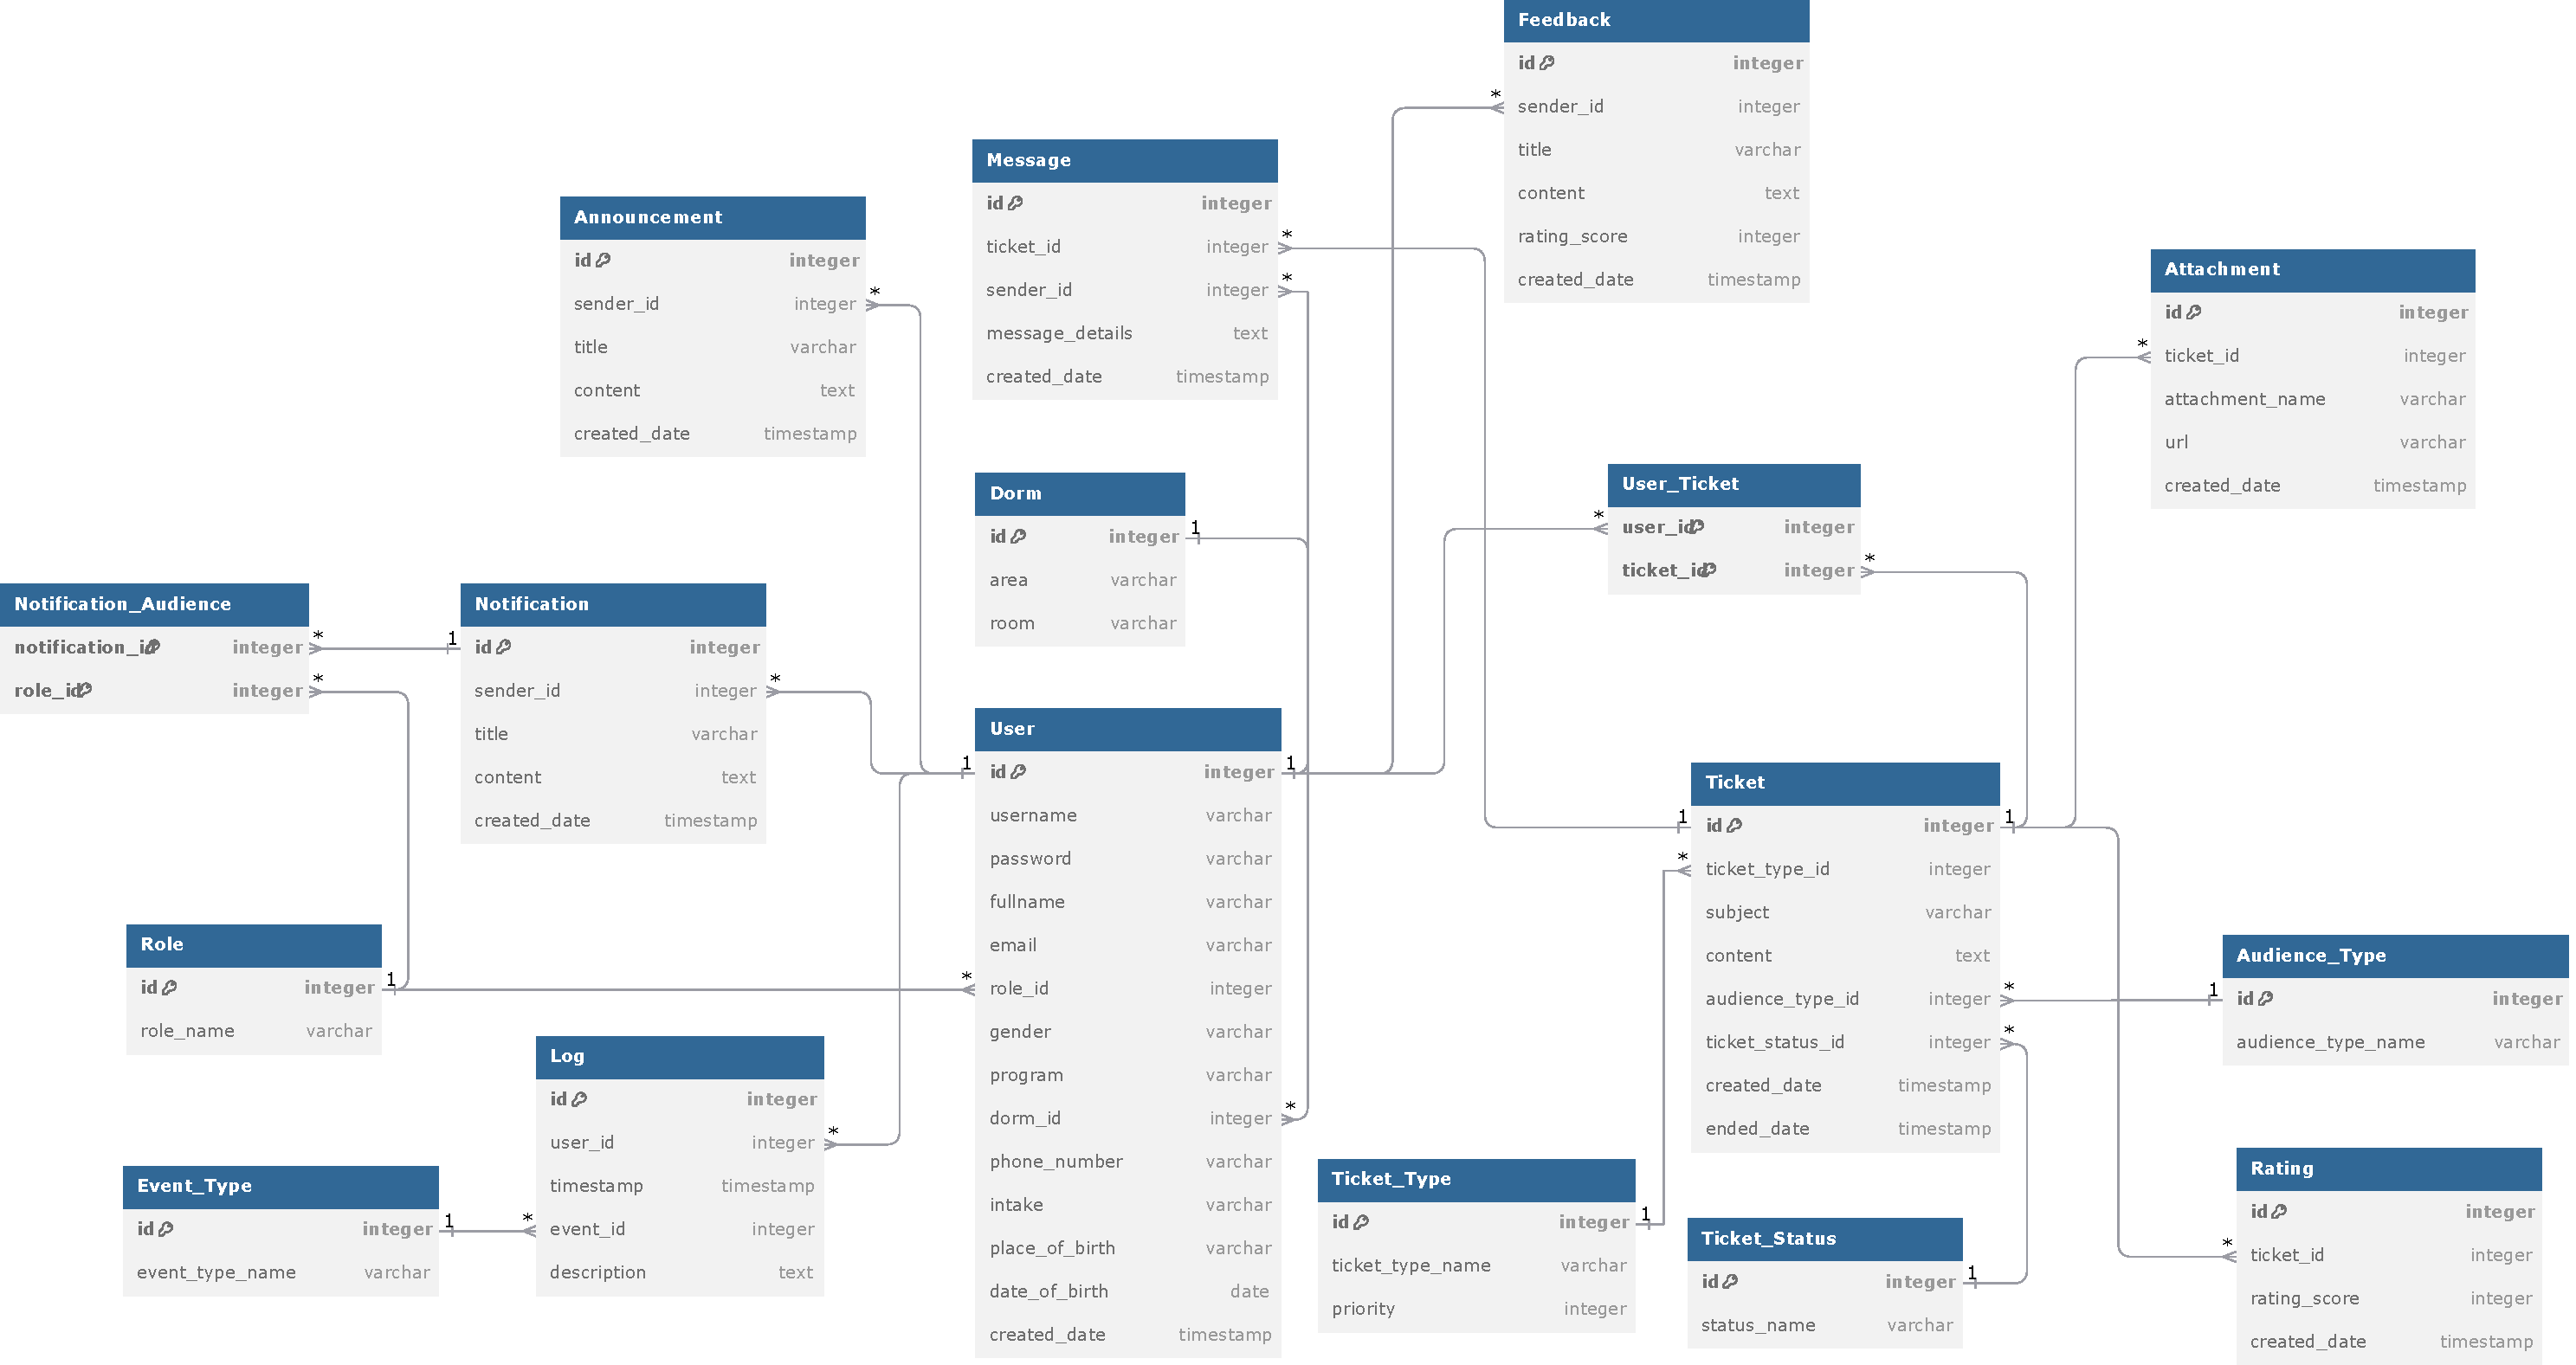
\includegraphics[width=1\columnwidth]{graphics/er-diagram.pdf}
		\caption{ER Diagram}
		\label{fig:er-diagram}
	\end{figure}


	\subsubsection{User Entity}


\subsection{System Architecture}

The system follows a three-tier architecture, consisting of the following layers:

\begin{figure}[H]
	\centering
	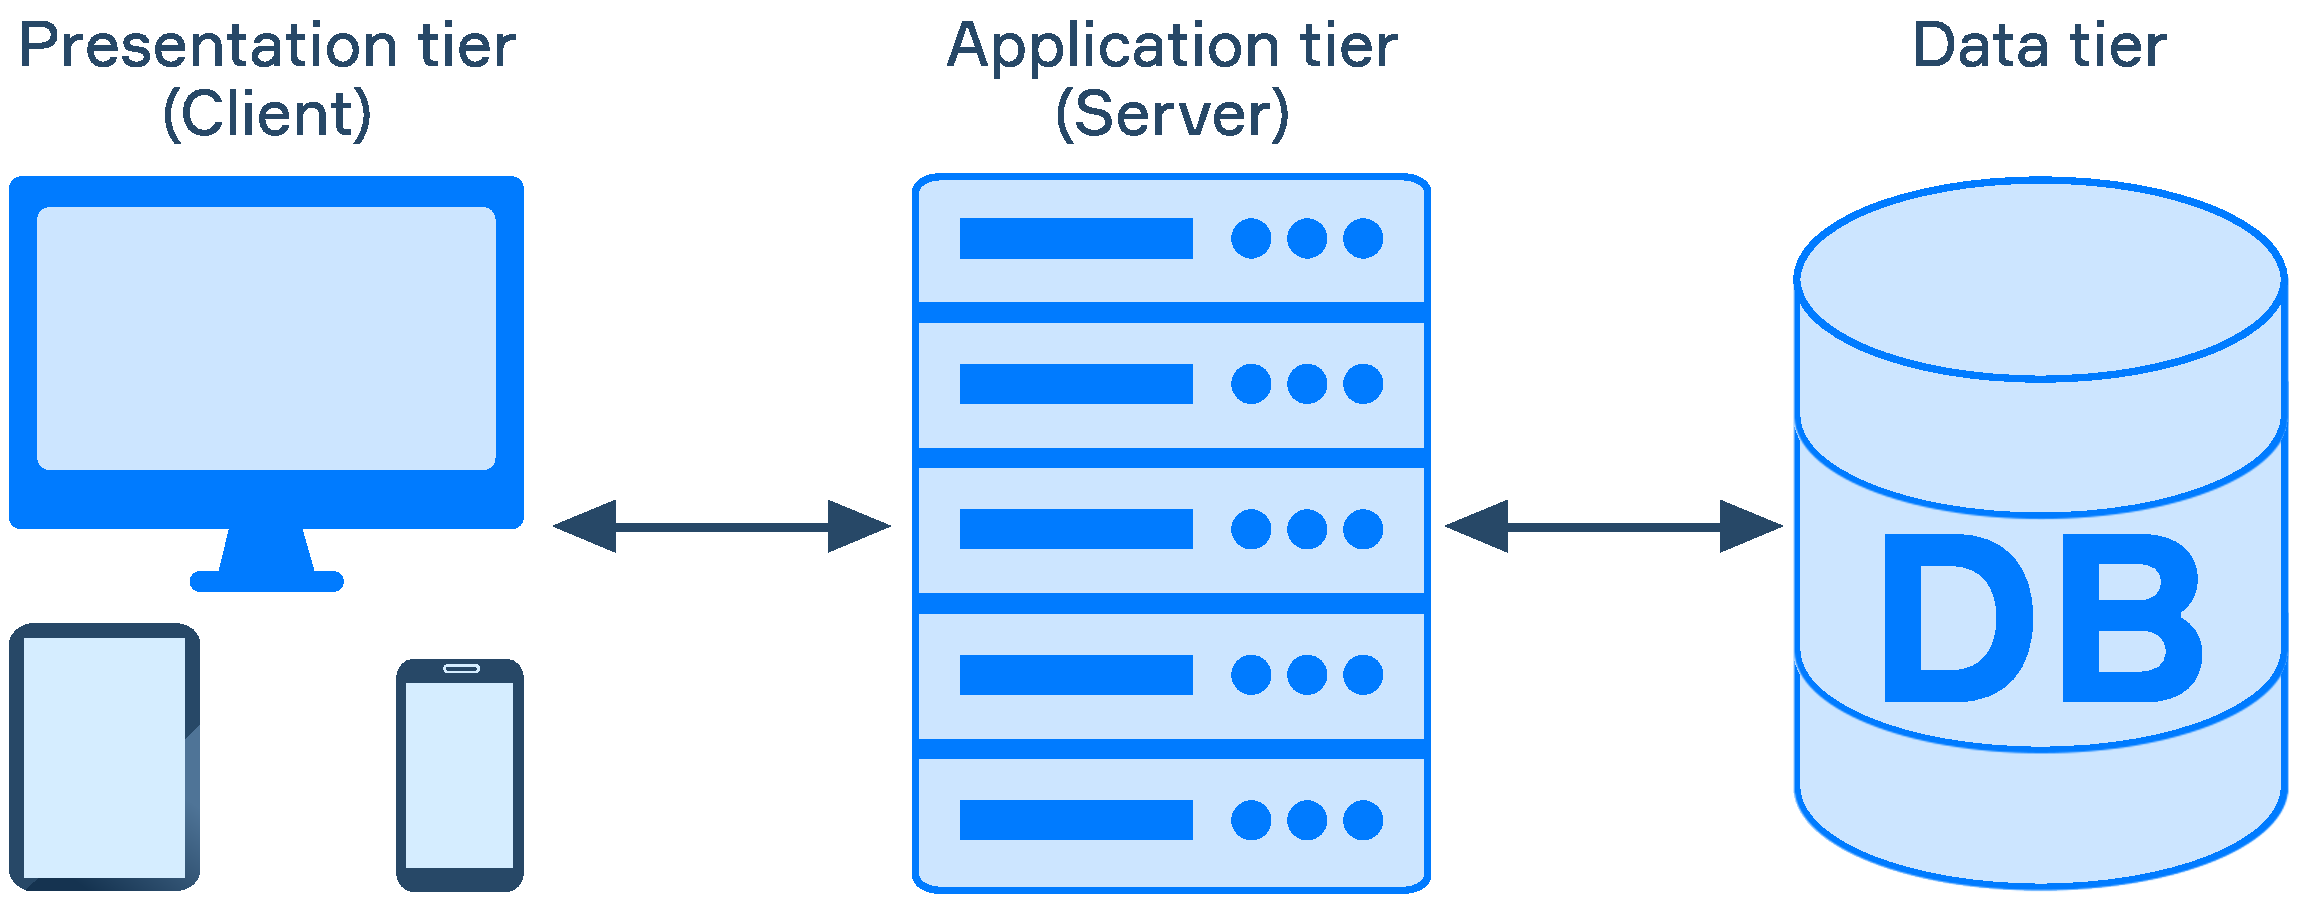
\includegraphics[width=0.7\columnwidth]{graphics/3-tier-arch.pdf}
	\caption{Three-tier Architecture \cite{3-tier}}
	\label{fig:3-tier}
\end{figure}


\begin{enumerate}
	\item \textbf{Presentation Layer (Client):}
	
	Handles all interactions with the user.
	Implements the user interface using ReactJS and Material UI.
	Communicates with the server through RESTful API calls and SocketIO for real-time features.
	Responsible for rendering components, collecting user input, and displaying data received from the backend.
	
	\item \textbf{Business Logic Layer (Server)}:
	
	NodeJS and ExpressJS handle the core business logic, such as processing support ticket requests, authenticating users, managing roles, and communicating with the database.
	SocketIO is used to manage real-time messaging between students and staff.
	Implements security features like JWT-based authentication and session management using Redis.
	
	\item \textbf{ Data Layer (Database)}:
	
	PostgreSQL stores all persistent data, including user profiles, support tickets, messages, and system logs.
	The server communicates with the database using SQL queries to retrieve, create, update, and delete records.
	Ensures data consistency and integrity by enforcing constraints, foreign keys, and relationships.
	
\end{enumerate}


\subsection{Frontend Design}












%	
	


	